\documentclass[tikz,border=10pt]{standalone}
\usepackage{amsmath}
\usepackage{tikz}
\usetikzlibrary{arrows.meta, positioning, calc, shapes.geometric}

\begin{document}
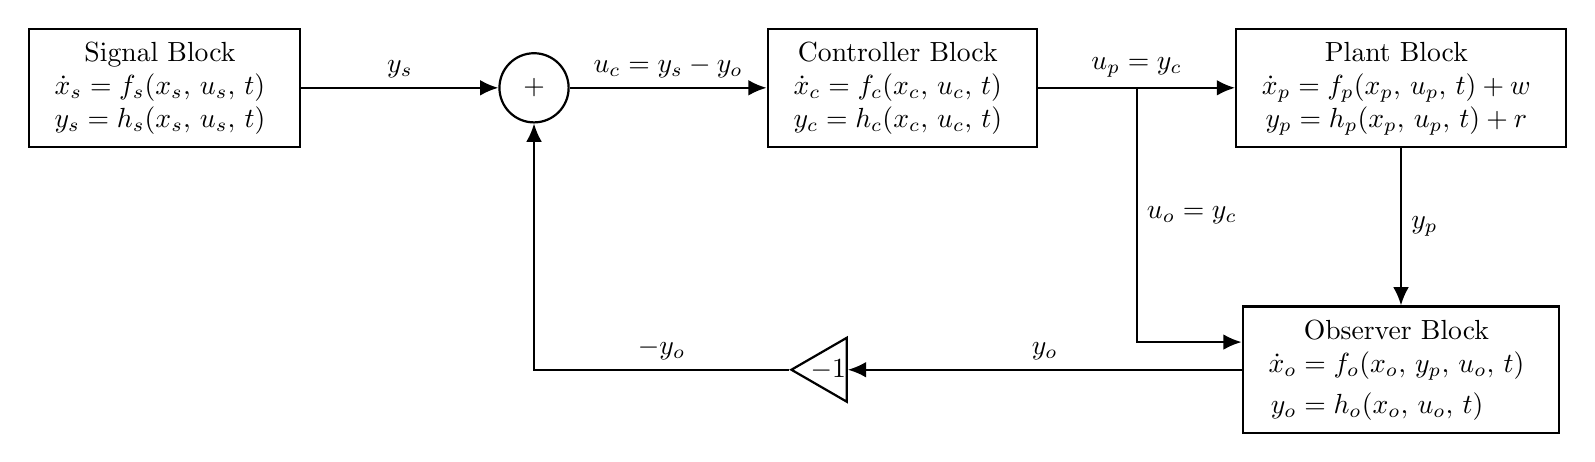
\begin{tikzpicture}[
  block/.style = {draw, thick, minimum height=3em, minimum width=6em, align=center},
  circ/.style  = {draw, circle, thick, minimum size=2.5em, inner sep=0pt},
  gain/.style  = {draw, isosceles triangle, isosceles triangle apex angle=60,
                  shape border rotate=135, % apex points LEFT
                  minimum height=2em, minimum width=2em, thick, inner sep=0pt},
  arrow/.style = {thick, -{Latex[width=2mm]}},
  node distance=2.5cm and 2.5cm
]

  % Signal Generator
  \node[block] (siggen) {
    \begin{tabular}{c}
      Signal Block \\
      $\dot{x}_s = f_s(x_s,\, u_s,\, t)$ \\
      $y_s = h_s(x_s,\, u_s,\, t)$
    \end{tabular}
  };

  % Summing junction (+)
  \node[circ, right=of siggen] (g) {$+$};

  % Controller
  \node[block, right=2.5cm of g] (controller) {
    \begin{tabular}{c}
      Controller Block\\
      $\dot{x}_c = f_c(x_c,\, u_c,\,t)$ \\
      $y_c = h_c(x_c,\, u_c,\,t)$
    \end{tabular}
  };

  % Plant
  \node[block, right=2.5cm of controller] (system) {
    \begin{tabular}{c}
      Plant Block \\
      $\dot{x}_p = f_p(x_p,\, u_p,\, t) + w$ \\
      $y_{p} = h_p(x_p,\, u_p,\, t) + r$
    \end{tabular}
  };

  % Observer
  \node[block, below=2cm of system] (observer) {
    \begin{tabular}{c}
  Observer Block \\
  $\begin{aligned}
    \dot{x}_o &= f_o(x_o,\, y_p,\, u_o,\, t) \\
    y_o       &= h_o(x_o,\, u_o,\, t)
  \end{aligned}$
\end{tabular}
  };

  % Gain -1 triangle, aligned to midpoint of observer.west (straight feed)
  \node[gain, anchor=east] (neg) at ($(observer.west)+(-5cm,0)$) {$-1$};

  % r -> +
  \draw[arrow] (siggen.east) -- node[above] {$y_s$} (g.west);

  % \hat{x} straight into triangle (no diagonal)
  \draw[arrow] (observer.west) -- node[above] {$y_o$} (neg.east);

  % Corner exactly under g: same x as g.south, same y as neg.west
  \coordinate (underG) at (g.south |- neg.west);

  % -\hat{x} exits apex (neg.west), goes to underG, then straight up into +
  \draw[arrow] (neg.west) -- node[above] {$-y_o$} (underG) -- (g.south);

  % e into controller
  \draw[arrow] (g.east) -- node[above] {$u_c = y_s - y_o$} (controller.west);

  % u to plant
  \draw[arrow] (controller.east) -- node[above] {$u_p = y_c$} (system.west);

  % u branch to observer
  \coordinate (usplit) at ($(controller.east)!0.5!(system.west)$);
  \coordinate[above=1em of observer.west] (observer_uin);
  \draw[arrow] (usplit) |- (observer_uin) node[pos=0.25, right]{$u_o=y_c$};

  % y to observer
  \draw[arrow] (system.south) -- node[right] {$y_p$} (observer.north);

\end{tikzpicture}
\end{document}
